\documentclass[a4paper,10pt]{article}
\usepackage[utf8]{inputenc}
\usepackage{babel}
\babelprovide[main,import=sr-Latn]{serbian}
\usepackage{amsmath}
\usepackage{amssymb}
\usepackage{microtype}
\usepackage{tikz}
\usepackage{hyperref}

\title{Implementacija metoda tabloa za iskaznu logiku}
\author{Jovan Škorić\\ 1030/2024}

\begin{document}

\maketitle

\begin{abstract}
Ovaj rad opisuje implementaciju metoda analitičkih tabloa za iskaznu
logiku. Metod tabloa je postupak odlučivanja koji zadovoljivost i
tautolo\-gičnost formule utvrđuje sistematskim pokušajem konstrukcije
(kontra)modela, razlaganjem formule na potformule po jednoobraznim
$\alpha$/$\beta$ pravilima. Predstavljamo teorijsku osnovu metoda,
opisujemo implementaciju u programskom jeziku C++ i ilustrujemo rad
programa na karakterističnim primerima.
\end{abstract}

\section{Uvod}
\label{sec:uvod}

Automatsko rezonovanje bavi se algoritmima koji mehanički utvrđuju da li
iz datih pretpostavki logički sledi neki zaključak. U srži mnogih takvih
algoritama nalazi se ispitivanje \emph{zadovoljivosti} i \emph{valjanosti}
formula. Za iskaznu logiku ovi problemi su odlučivi, ali naivno ispitivanje
svih valuacija zahteva $2^n$ koraka za formulu sa $n$ iskaznih slova, pa se
troši rad i na grane koje su očigledno beznadežne.

Metod analitičkih tabloa (engl.\ \emph{analytic tab\-leaux}) valjanost formule
ispituje sistematskim pokušajem konstrukcije \emph{kontramodela} --- valuacije
koja formulu obara. Umesto nabrajanja svih valuacija, formula se razlaže na
potformule po malom skupu jednoobraznih pravila, čime se beznadežne grane
pretrage rano odsecaju. Ako nijedan kontramodel ne postoji, formula je valjana.
Metod je u današnjem obliku uveo Smullyan \cite{smullyan}, oslanjajući se na
ranije radove Beta i Hintike, a danas je jedna od standardnih tehnika u
automatskom dokazivanju teorema \cite{fitting, dagostino}. Prednost u odnosu na
metod rezolucije jeste u tome što tablo radi neposredno nad izvornom formulom,
bez prethodnog prevođenja u normalnu formu, i što se prirodno uopštava na
predikatsku i modalne logike.

Ostatak ovog rada organizovan je na sledeći način. U poglavlju
\ref{sec:osnove} navodimo osnovne pojmove iskazne logike i notaciju.
U poglavlju \ref{sec:opis_metode} dajemo opis metoda tabloa. Poglavlje
\ref{sec:implementacija} sadrži detalje implementacije. Najzad,
poglavlje \ref{sec:zakljucak} sadrži zaključna razmatranja.

\section{Osnove}
\label{sec:osnove}

U ovom poglavlju uvodimo sintaksu i semantiku iskazne logike, kao i pojmove
zadovoljivosti, valjanosti i SAT problema, koji se koriste u ostatku rada.

\paragraph{Sintaksa.}
Neka je $\mathcal{P} = \{p, q, r, \dots\}$ prebrojiv skup \emph{iskaznih slova}
(atoma). Skup \emph{iskaznih formula} definiše se induktivno:
\begin{itemize}
 \item logičke konstante $\top$ (tačno) i $\bot$ (netačno) su formule;
 \item svako iskazno slovo $p \in \mathcal{P}$ je formula;
 \item ako su $A$ i $B$ formule, onda su i $\neg A$, $(A \wedge B)$,
       $(A \vee B)$, $(A \rightarrow B)$ i $(A \leftrightarrow B)$ formule.
\end{itemize}
\emph{Potformula} formule je svaka formula upotrebljena u njenoj izgradnji.

\paragraph{Semantika.}
\emph{Valuacija} je preslikavanje $v : \mathcal{P} \to \{0,1\}$ koje svakom
iskaznom slovu dodeljuje istinitosnu vrednost. Ono se jednoznačno proširuje do
preslikavanja $I_v$ definisanog nad svim formulama:
\begin{align*}
 I_v(\top) &= 1, & I_v(\bot) &= 0, \\
 I_v(p) &= v(p), & I_v(\neg A) &= 1 - I_v(A), \\
 I_v(A \wedge B) &= \min\big(I_v(A), I_v(B)\big), &
 I_v(A \vee B) &= \max\big(I_v(A), I_v(B)\big), \\
 I_v(A \rightarrow B) &= \max\big(1 - I_v(A),\, I_v(B)\big), &
 I_v(A \leftrightarrow B) &= 1 \text{ akko } I_v(A) = I_v(B).
\end{align*}
Ako je $I_v(A) = 1$, kažemo da je formula $A$ \emph{tačna} pri valuaciji $v$ i
da je $v$ \emph{model} formule $A$, u oznaci $v \models A$.

\paragraph{Zadovoljivost i valjanost.}
Formula je \emph{zadovoljiva} ako ima bar jedan model; u suprotnom je
\emph{nezadovoljiva} (kontradikcija). Formula $A$ je \emph{valjana}
(tautologija) ako je tačna pri svakoj valuaciji, u oznaci $\models A$. Ova dva
pojma povezuje dualnost koju metod tabloa neposredno koristi:
\begin{equation}
 \label{eq:dualnost}
 {\models} A \quad \text{akko} \quad \neg A \text{ je nezadovoljiva}.
\end{equation}

\paragraph{SAT problem.}
\emph{Problem iskazne zadovoljivosti} (SAT) jeste problem odlučivanja da li je
data iskazna formula zadovoljiva. To je prvi problem za koji je dokazano da je
NP-kompletan (Cook--Levin), pa se za njega ne očekuje algoritam polinomijalne
složenosti. Ispitivanje valjanosti je, po dualnosti~\eqref{eq:dualnost},
komplementaran problem i svodi se na SAT preko negacije formule.

\section{Opis metode}
\label{sec:opis_metode}

Metod tabloa valjanost formule svodi na pokušaj konstrukcije kontramodela.
Da bi se u toku konstrukcije pratile pretpostavke o istinitosnim vrednostima
potformula, formule se \emph{označavaju}.

\paragraph{Označene formule.}
\emph{Označena formula} je izraz oblika $T\varphi$ ili $F\varphi$, gde je
$\varphi$ iskazna formula. Oznaka $T$ predstavlja pretpostavku da je $\varphi$
tačna, a $F$ da je netačna; formalno, uz valuaciju $v$ važi
$I_v(T\varphi) = I_v(\varphi)$ i $I_v(F\varphi) = 1 - I_v(\varphi)$. Dokaz da je
formula $A$ tautologija počinje od korena $FA$: pretpostavimo da $A$ nije tačna
i pokušamo tu pretpostavku da razvijemo do konkretne valuacije.

\paragraph{Pravila razlaganja.}
Sva pravila svode se na dva tipa. \emph{Konjunktivna} ($\alpha$) pravila
proširuju granu sa \emph{obe} komponente, dok \emph{disjunktivna} ($\beta$)
pravila granu \emph{račvaju} na dve. Ova jednoobrazna (Smuljanova) notacija
data je u sledećim tabelama:
\begin{center}
\begin{tabular}{c|cc}
$\alpha$ & $\alpha_1$ & $\alpha_2$ \\ \hline
$T(A \wedge B)$ & $TA$ & $TB$ \\
$F(A \vee B)$ & $FA$ & $FB$ \\
$F(A \rightarrow B)$ & $TA$ & $FB$ \\
$T\neg A$ & $FA$ & \\
$F\neg A$ & $TA$ & \\
\end{tabular}
\qquad
\begin{tabular}{c|cc}
$\beta$ & $\beta_1$ & $\beta_2$ \\ \hline
$F(A \wedge B)$ & $FA$ & $FB$ \\
$T(A \vee B)$ & $TA$ & $TB$ \\
$T(A \rightarrow B)$ & $FA$ & $TB$ \\
& & \\
& & \\
\end{tabular}
\end{center}
Ekvivalenciju razlažemo takođe kao $\beta$ pravilo, ali sa parovima komponenti:
$T(A \leftrightarrow B)$ grana se na $\{TA, TB\}$ i $\{FA, FB\}$, a
$F(A \leftrightarrow B)$ na $\{TA, FB\}$ i $\{FA, TB\}$. Za logičke konstante:
grana koja sadrži $F\top$ ili $T\bot$ odmah se zatvara, dok se $T\top$ i $F\bot$
uvek zadovoljavaju i uklanjaju.

\paragraph{Konstrukcija i zatvaranje.}
Tablo je stablo označenih formula. Gradi se tako što se na tekućoj grani bira
još neiskorišćena formula i na nju primeni odgovarajuće $\alpha$ ili $\beta$
pravilo, pri čemu se nove formule dopisuju na kraj svih grana koje kroz nju
prolaze. Grana se \emph{zatvara} čim sadrži $T\varphi$ i $F\varphi$ za istu
formulu $\varphi$ (očigledna protivrečnost), a \emph{otvorena} je ako je
kompletirana bez takve protivrečnosti. Tablo je \emph{zatvoren} ako su mu sve
grane zatvorene. Odatle slede dve procedure odlučivanja:
\begin{itemize}
 \item \textbf{valjanost} formule $A$: koren je $FA$; ako se tablo zatvori,
       $A$ je tautologija, a inače svaka otvorena grana daje kontramodel;
 \item \textbf{zadovoljivost} formule $A$: koren je $TA$; svaka otvorena grana
       daje model, a ako se tablo zatvori, $A$ je nezadovoljiva.
\end{itemize}
Radi efikasnosti, $\alpha$ pravila primenjuju se pre $\beta$ pravila: pošto
$\alpha$ ne račva stablo, odlaganje račvanja daje manji tablo.

\paragraph{Primer.}
Slika~\ref{fig:tablo} prikazuje zatvoren tablo za formulu
$(p \rightarrow q) \rightarrow (\neg q \rightarrow \neg p)$ (zakon kontrapozicije).
Koren je označen sa $F$; uzastopnom primenom $\alpha$ pravila dobijaju se
literali $Fq$ i $Tp$, a razlaganje $T(p \rightarrow q)$ (jedino $\beta$ pravilo)
račva stablo na $Fp$ i $Tq$. Obe grane sadrže protivrečan par ($Tp/Fp$, odnosno
$Fq/Tq$), pa se zatvaraju. Kako se ceo tablo zatvorio, formula je tautologija.

\begin{figure}[ht]
\centering
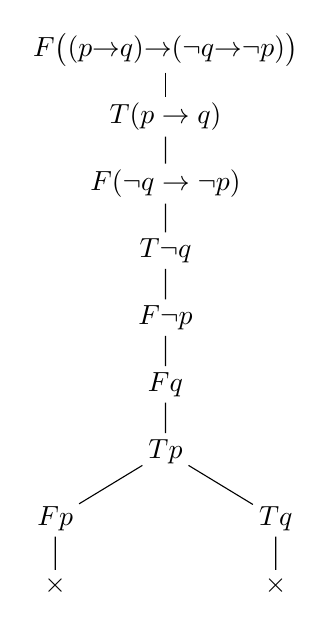
\begin{tikzpicture}[level distance=8.5mm, sibling distance=28mm,
                    every node/.style={inner sep=2pt}]
\node {$F\big((p{\rightarrow}q){\rightarrow}(\neg q{\rightarrow}\neg p)\big)$}
 child { node {$T(p \rightarrow q)$}
  child { node {$F(\neg q \rightarrow \neg p)$}
   child { node {$T\neg q$}
    child { node {$F\neg p$}
     child { node {$Fq$}
      child { node {$Tp$}
       child { node {$Fp$} child { node {$\times$} } }
       child { node {$Tq$} child { node {$\times$} } }
      }
     }
    }
   }
  }
 };
\end{tikzpicture}
\caption{Zatvoren tablo za zakon kontrapozicije. Simbol $\times$ označava
zatvorenu granu.}
\label{fig:tablo}
\end{figure}

\paragraph{Zaustavljanje, korektnost i kompletnost.}
Svako pravilo zamenjuje označenu formulu njenim pravim potformulama, pa broj
veznika strogo opada; zato je svaka konstrukcija konačna. \emph{Korektnost}:
ako se tablo sa korenom $FA$ zatvori, formula $\neg A$ je nezadovoljiva, pa je
$A$ valjana. \emph{Kompletnost}: svaka otvorena završena grana čini
\emph{Hintikin skup}, koji je uvek zadovoljiv; stoga, ako je $A$ tautologija,
nijedna grana ne može ostati otvorena, tj.\ tablo se nužno zatvara. Detaljni
dokazi ovih tvrđenja dati su u \cite{smullyan, fitting}.

\section{Implementacija}
\label{sec:implementacija}

\paragraph{Jezik i alati.}
Metod je implementiran u programskom jeziku C++ (standard C++17), bez ikakvih
spoljašnjih biblioteka --- koristi se isključivo standardna biblioteka. Za
prevođenje su dovoljni prevodilac \texttt{g++} i \texttt{GNU make}.

\paragraph{Organizacija koda.}
Kôd je podeljen na module prema odgovornosti:
\begin{itemize}
 \item \texttt{formula.hpp} --- apstraktno sintaksno stablo (AST) formule;
 \item \texttt{parser.\{hpp,cpp\}} --- leksička i sintaksna analiza ulaza;
 \item \texttt{signed\_formula.hpp} --- označene formule i $\alpha$/$\beta$
       klasifikacija;
 \item \texttt{tableau.\{hpp,cpp\}} --- konstrukcija tabloa i procedure
       odlučivanja;
 \item \texttt{main.cpp} --- komandnolinijski interfejs.
\end{itemize}

\paragraph{Reprezentacija formule.}
Formula je predstavljena kao \texttt{std::variant} pet slučajeva
(\texttt{False}, \texttt{True}, \texttt{Atom}, \texttt{Not}, \texttt{Binary}),
a čvorovi se dele preko pametnog pokazivača \texttt{std::shared\_ptr} (tip
\texttt{FormulaPtr}), čime se izbegava ručno upravljanje memorijom. Pomoćne
funkcije \texttt{is<T>} i \texttt{as<T>} obavljaju bezbedno ispitivanje i
izdvajanje varijante.

\paragraph{Parser.}
Ulaz se najpre deli na tokene (\texttt{tokenize}), a zatim se rekurzivnim
spustom gradi AST. Prioritet veznika kodiran je redosledom poziva funkcija:
$\neg$ (najviši), pa $\wedge$, $\vee$, $\rightarrow$, $\leftrightarrow$
(najniži); pri tom su $\rightarrow$ i $\leftrightarrow$ desno, a $\wedge$ i
$\vee$ levo asocijativni. Neispravan ulaz signalizira se izuzetkom
\texttt{ParseError}, koji se hvata na granici sistema, u \texttt{main.cpp}.

\paragraph{Klasifikacija pravila.}
Funkcija \texttt{classify} preslikava označenu formulu u strukturu
\texttt{Expansion}, čije polje \texttt{kind} uzima jednu od vrednosti
\texttt{Alpha}, \texttt{Beta}, \texttt{Literal}, \texttt{Closed} ili
\texttt{Satisfied}. Time je cela tabela pravila iz
poglavlja~\ref{sec:opis_metode} sabijena u jednu funkciju, pa ostatak
algoritma ne mora da poznaje pojedinačne veznike.

\paragraph{Jezgro algoritma.}
Zatvaranje jedne grane ispituje rekurzivna funkcija \texttt{closes}. Ona
održava radnu listu složenih formula (\texttt{work}) i delimičnu valuaciju
literala (tip \texttt{Valuation}, tj.\ \texttt{std::map<std::string,bool>}).
Pomoćna funkcija \texttt{place} smešta formulu na granu: literal upisuje u
valuaciju i pri tom otkriva protivrečnost (isti atom sa suprotnim znakom),
dok složene formule odlaže u \texttt{work}. Funkcija \texttt{pickIndex} bira
sledeću formulu tako da $\alpha$ pravila imaju prednost nad $\beta$, čime se
stablo drži malim. Kod $\beta$ račvanja grana se zatvara samo ako se
\emph{sve} opcije zatvore; čim se naiđe na otvorenu granu, njena valuacija
vraća se kao (kontra)model. Javne funkcije \texttt{isValid} i
\texttt{isSatisfiable} postavljaju odgovarajući koren ($Ff$ odnosno $Tf$) i
pozivaju jezgro, a \texttt{printValidityTableau} i
\texttt{printSatisfiabilityTableau} ispisuju celo stablo radi ilustracije.

\paragraph{Prevođenje i pokretanje.}
Projekat se prevodi komandom \texttt{make}, a program se poziva ovako:
\begin{verbatim}
make                             # prevodi u build/tablo
./build/tablo valid "(p -> q) -> (~q -> ~p)"
./build/tablo sat "(p | q) & (~p | r)" --tree
./build/tablo                    # ugradjeni demo primeri
\end{verbatim}
Režim \texttt{valid} ispituje tautologičnost, \texttt{sat} zadovoljivost, a
opcija \texttt{--tree} dodatno iscrtava konstruisani tablo. Za prevođenje je
potreban prevodilac sa podrškom za C++17 (npr.\ \texttt{g++} verzije 7 ili
novije) i \texttt{GNU make}.

\paragraph{Primeri korišćenja.}
Sledeći isečak prikazuje tipičan rad programa:
\begin{verbatim}
$ ./build/tablo valid "(p -> q) -> (~q -> ~p)"
(p -> q) -> (~q -> ~p)  =>  TAUTOLOGIJA

$ ./build/tablo valid "p -> q"
p -> q  =>  NIJE TAUTOLOGIJA, kontramodel {p=1, q=0}

$ ./build/tablo sat "(p | q) & (~p | r)"
(p | q) & (~p | r)  =>  ZADOVOLJIVA, model {p=1, r=1}

$ ./build/tablo sat "p -> q" --tree
p -> q  =>  ZADOVOLJIVA, model {p=0}

T (p -> q)
|-- F p
|   o (otvorena) {p=0}
`-- T q
    o (otvorena) {q=1}
\end{verbatim}
Prva dva poziva ilustruju dualnost: za formulu koja nije tautologija program
vraća kontramodel koji je obara. U poslednjem primeru opcija \texttt{--tree}
prikazuje konstruisani tablo --- koren $T(p \rightarrow q)$ je $\beta$ formula,
pa se grana na $Fp$ i $Tq$; obe grane ostaju otvorene i daju po jedan model, a
oznaka \texttt{o} obeležava otvorenu granu.

\section{Zaključak}
\label{sec:zakljucak}

U ovom radu implementiran je metod analitičkih tabloa za iskaznu logiku i
opisana je njegova teorijska osnova. Program, napisan u jeziku C++, za
proizvoljnu iskaznu formulu odlučuje njenu tautologičnost i zadovoljivost i,
po potrebi, konstruiše (kontra)model ili ispisuje ceo tablo.

Glavna prednost metoda jeste to što radi neposredno nad izvornom formulom, bez
prevođenja u normalnu formu, i što se otvorena grana prirodno čita kao model.
Kao i svi postupci za SAT, metod u najgorem slučaju ima eksponencijalnu
složenost; prikazana implementacija koristi osnovnu heuristiku prioriteta
$\alpha$ nad $\beta$ pravilima, dok naprednije varijante (na primer KE-tablo
ili sprega sa DPLL pretragom) mogu dodatno smanjiti veličinu stabla. Budući da
se pravila razlaganja lako uopštavaju, isti okvir prirodno se proširuje na
predikatsku i modalne logike, što metod tabloa čini korisnim i izvan iskazne
logike.

\begin{thebibliography}{100}
\bibitem{smullyan} Smullyan, Raymond M. \emph{First-Order Logic}.
Springer-Verlag, 1968.
\bibitem{fitting} Fitting, Melvin. \emph{First-Order Logic and Automated
Theorem Proving}. 2nd ed., Springer, 1996.
\bibitem{dagostino} D'Agostino, Marcello, et al., eds. \emph{Handbook of
Tableau Methods}. Kluwer Academic Publishers, 1999.
\end{thebibliography}

\end{document}
